For each of the afforementioned passages the throughflow was computed. This is done using a simple integration to calculate the volumetric flux through each passage.
\begin{align}
	Q = \int \int_A \vec{u} \cdot d\vec{A}
\end{align}	
For each passage a suitible location was chosen such that there are no boundaries next to the passageways. Then the $u$ component of the flow is used to compute the total flow. This method is the same for each of the passages and thus we can study the effect of changes in bathymetry to on the relative strenght of the flow. However, it should be noted that these values may not represent real physical values. As the passages are often only a few gridcells wide and, the nature of the 4 degree model. Resulting in discepencies due to boundary conditions. The passageways have been labeled in figure (figure of these) and results are plotted in figure (figure of these).

\begin{figure}[H]
	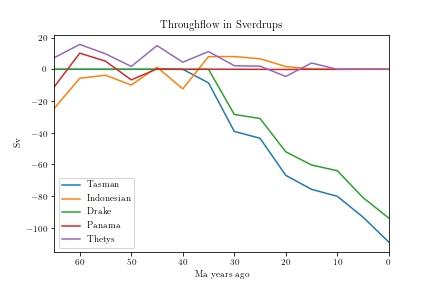
\includegraphics[width=\linewidth]{throughflow}
<<<<<<< HEAD
	\caption{Passage throughflow in Sverdrups}
	\label{fig:tfpassages}
\end{figure}
=======
	\caption{test caption}
	\label{fig:throughflow}
\end{figure}

To get a better understanding of the flows we can look at a vector field showing the direction of horizontal water displacement. This is done by making a weighted mean of the horizontal flow field for each layer. Weighted by the volume of each grid cell. In this way each arrow actualy represents relative flow velocity compared to other gridpoints.

%TODO add figure of flow
>>>>>>> d0f1558adfd0e33ebb91ee82f52c66990edbfb0d
